\documentclass{beamer}
\usetheme{Warsaw}
\usepackage[utf8]{inputenc}
\usepackage[T1]{fontenc}

\usepackage{svg}
\setsvg{inkscape = inkscape -z -D}


\title[DNNLM]{Deep Neural Network Language Models}
\author[A. Peyrard, T. Cantenot]{Alex Peyrard, Thierry Cantenot}
\institute{Shanghai JiaoTong University}
\date{\today}

\addtobeamertemplate{footline}{\insertframenumber/\inserttotalframenumber}

\begin{document}
\begin{frame}[plain]
	  \titlepage
\end{frame}

\begin{frame}{Introduction}
	\begin{center}
		Deep Neural Networks Language Models\\
		Ebru Arısoy, Tara N. Sainath, Brian Kingsbury, Bhuvana Ramabhadran\\
		IBM T.J. Watson Research Center\\
		Yorktown Heights, NY, 10598, USA\\
		\{earisoy, tsainath, bedk, bhuvana\}@us.ibm.com
	\end{center}
\end{frame}

\begin{frame}{What is a Language Model?}
	\begin{quote}
		A statistical language model assigns a probability to a sequence of m words $P(w_1,\ldots,w_m)$ by means of a probability distribution. \\ \flushright\emph{Wikipedia -- Language Models}
	\end{quote}
\end{frame}

\begin{frame}{What is a Neural Network?}
	\begin{figure}[!ht]
		\centering
		\rule{0cm}{0cm}
		\includesvg[width = 0.5\textwidth, svgpath=images/]{ANN}
		\caption{A neural network}
	\end{figure}
\end{frame}

\begin{frame}{What is a Neural Network?}
	A neuron is defined by :
	\begin{itemize}
		\item Bias
		\item Weight
		\item Activation function
	\end{itemize}
	\vspace{5mm}
	The bias and weight are updated during training. The activation function is chosen when the network is first designed.\\
	\vspace{5mm}
	Thus, the output of a node is
	\[f(\sum\limits_{i}W_{i}x_{i} + b)\]
\end{frame}

\begin{frame}{Activation function}
	The activation function often if the sigmoid or hyperbolic tangent function.
	\begin{center}
		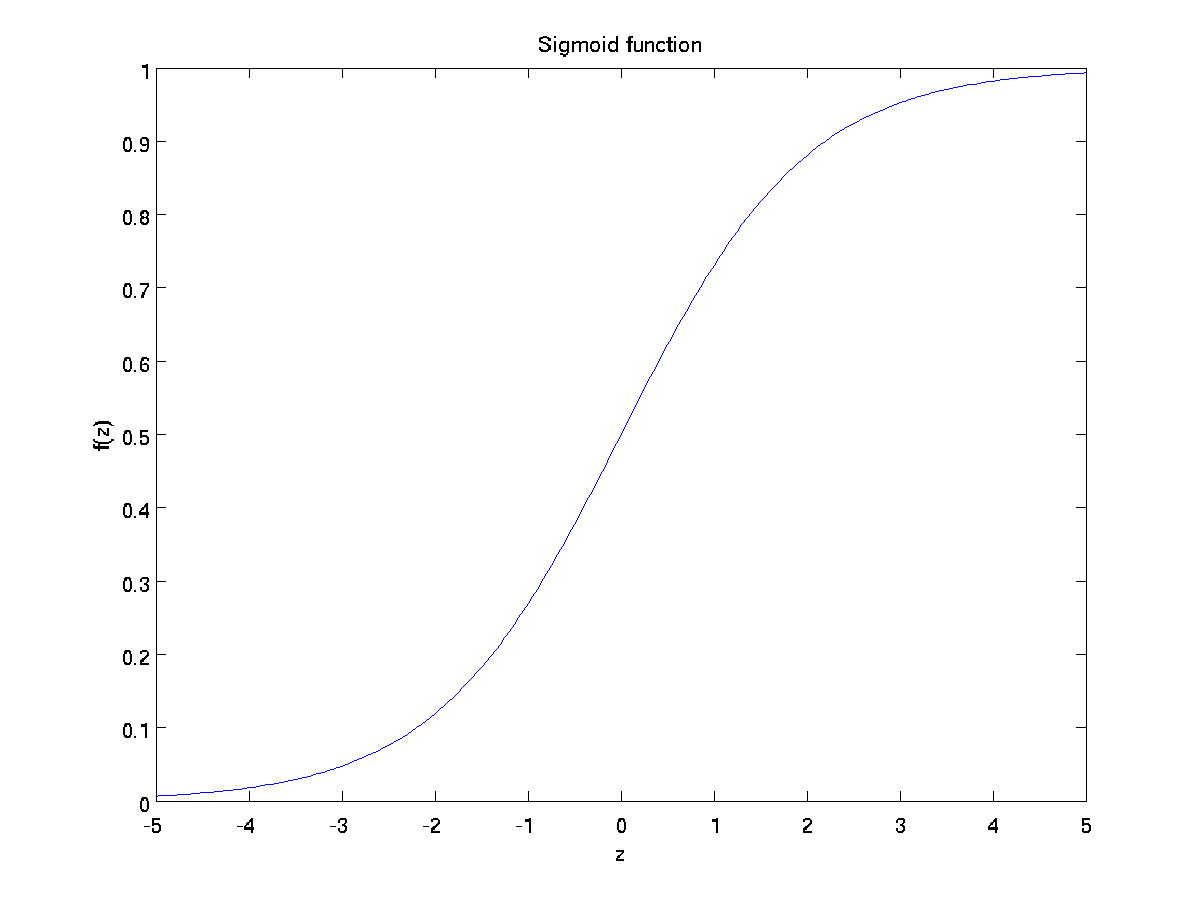
\includegraphics[scale=0.28]{images/sigmoid.png}
		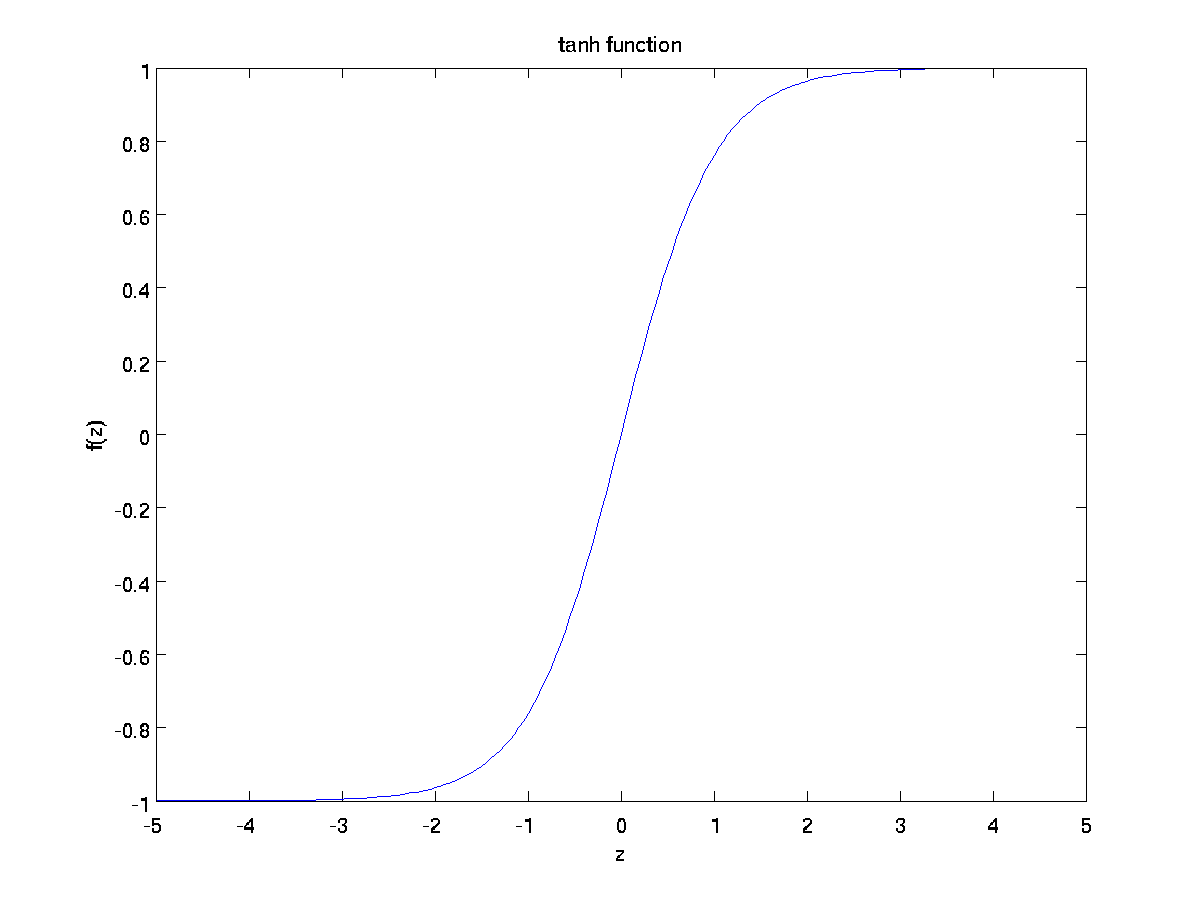
\includegraphics[scale=0.28]{images/tanh.png}
	\end{center}
\end{frame}

\end{document}
